\documentclass[a4paper, 12pt]{report}

\usepackage[utf8]{inputenc}
\usepackage[T1]{fontenc}
\usepackage[french]{babel} 
\usepackage[top=35mm, bottom=35mm, left=25mm, right=25mm]{geometry}
\usepackage{geometry}
\usepackage{graphicx}
\usepackage{multirow}  
\usepackage{subfigure}
\usepackage{verbatim}
\usepackage{url}
\usepackage{algorithmic, algorithm} 
\usepackage{amsmath,amsfonts,amssymb}
\usepackage{lmodern}
\usepackage{microtype}
\usepackage{xcolor}
\usepackage{textcomp}
\usepackage{framed}
\usepackage{tcolorbox}
\usepackage{etoolbox}
\usepackage{hyperref}

\definecolor{vert}{RGB}{56, 155, 34}
\definecolor{rouge}{RGB}{157, 29, 29}


\hypersetup{
    colorlinks,
    citecolor=black,
    filecolor=black,
    linkcolor=black,
    urlcolor=black,
}

\title{Analyse d'applets JavaCard et réalisation d'automates}
\author{Romain \bsc{Barrat}
  \and
  Simon \bsc{Garrelou}
  \and
  Clément \bsc{Jarrige}
  \and
  Marouan \bsc{Sami} \and
  ~\and
  Encadrant : Jean-Louis \bsc{Lanet}}

\date{13 janvier 2017}


\setcounter{secnumdepth}{3}
\usepackage{fancyhdr}
\pagestyle{fancy}
 \lhead{\leftmark}
 \rhead{}

 
%création du glossaire
%Création des doubles entrées acronyme-glossaire
\usepackage{xparse}

\usepackage[acronym]{glossaries}

\makeglossaries

\DeclareDocumentCommand{\newdualentry}{ O{} O{} m m m m } {
  \newglossaryentry{gls-#3}{name={#5},text={#5\glsadd{#3}},
    description={#6},#1
  }
  \newacronym[see={[Glossary:]{gls-#3}},#2]{#3}{#4}{#5\glsadd{gls-#3}}
}

%exemple d'entrée double :
%\newdualentry{OWD} % label
%  {OWD}            % abbreviation
%  {One-Way Delay}  % long form
%  {The time a packet uses through a network from one host to another}



\newdualentry{VM}
    {VM}
    {machine virtuelle}
    { ou Virtual Machine en anglais est une machine (un ordinateur par exemple) simulée par un autre équipement.}
    

\newglossaryentry{GNU-Linux}
{
        name=GNU-Linux,
        description={ est le nom associé à un système d'exploitation alliant le noyau Linux, développé par Linus Torvalds, et les outils du projet GNU initié par Richard M. Stallman.}
}

\newglossaryentry{microsoft}
{
        name=Microsoft,
        description={ est une entreprise fondée en 1975 par Bill Gates spécialisée dans la conception de logiciels informatique.}
}

\newglossaryentry{windows}
{
        name=Windows,
        description={ est le principal système d'exploitation développé par Microsoft.}
}

 




\begin{document}
	\begin{titlepage}
\begin{center}

    
\includegraphics[width=0.5\textwidth]{images/logo-ul.png} ~\\[1cm]
    \textsc{\LARGE Faculté des Sciences et Techniques} \\[0.5cm]
    \textsc{\Large Département Informatique} \\[1.5cm]

    % Titre
    \vspace*{3,5cm}

    \hrule height 0.05cm ~\\[0.4cm]
    {\huge \bfseries Analyse et développement logiciel} \\[0.5cm]
    {\LARGE \bfseries Analyse d'applets JavaCard et réalisation d'automates} \\[0.5cm]
    \hrule height 0.05cm ~\\[0.6cm]

    {\large Romain \bsc{Barrat} ---
	Simon \bsc{Garrelou} ---
	Clément \bsc{Jarrige} ---
	Marouan \bsc{Sami} }

    ~\\[2cm]


    % Footer
    \vfill
    Encadrant : 	\bsc{Lanet} Jean-Louis \\
	Responsable Module : \bsc{Crespin} Benoît\\
    {\large  2016 - 2017 \\}

\end{center}
\end{titlepage}

	\newpage
	~
	\thispagestyle{empty}
	
	\chapter*{Introduction}

\paragraph{}
Au cours de notre premier semestre de master Informatique, nous avons eu à choisir un sujet de projet qui sera à traiter tout au long de l'année.
Etant quatre étudiants nous dirigeant vers le master \bsc{Cryptis}, nous avons choisi de prendre un sujet en lien avec la sécurité informatique, et notamment avec la sécurité des cartes à puces fonctionnant sous JavaCard.

\paragraph{Choix du projet}
Sous l'impulsion de Monsieur Jean-Louis \bsc{Lanet}, nous avons donc choisi le projet intitulé ``Analyse d'applets JavaCard et réalisation d'automates''.

\paragraph{Objectif du projet}
L'objectif du projet est d'être capable de réaliser une application permettant de générer, à partir du code source d'une applet JavaCard, un automate ayant le même fonctionnement que l'applet en question. Cette opération aura pour objectif de pouvoir tester, en simulant un fonctionnement réel via l'automate, l'applet jusque dans ces détails et ainsi révéler d'éventuelles failles de sécurité.

\paragraph{Déroulement du projet}
Dans ce rapport préliminaire, nous allons vous présenter comment et avec quels outils nous comptons, au semestre prochain, atteindre notre objectif.

Nous commenceront par présenter quelle(s) technologie(s) déjà existante(s) réalise(nt) ou approche(nt) des travaux en lien avec notre objectif. Puis nous présenterons un outil qui permet d'utiliser la technique des exécutions concoliques dans le but de tester des applications, viendra ensuite les moyens de réalisation d'un automate généré grâce aux tests et enfin le stockage des graphes liés à l'automate généré.

Une dernière partie consistera à présenter le travail à réaliser lors du prochain semestre.
	\newpage
	\tableofcontents

        \chapter{Bandera~: génération de modèles à partir de code source Java}

\paragraph{}
Bandera~\cite{bandera1} est un logiciel permettant d'analyser un
projet Java et d'en extraire un modèle utilisable par un vérificateur
de modèle. Il a été développé suite à la collaboration de chercheurs de
l'Université d'Hawaï et de l'Université d'État du Kansas.

\paragraph{}
Ce logiciel n'est plus maintenu depuis 2005, néanmoins il peut être
intéressant de voir les décisions prises par ses développeurs pour
réaliser ce programme, en effet notre projet possède certaines
similarités~: nous cherchons aussi à analyser du code source Java afin
d'en extraire un automate.

\paragraph{}
La vérification de modèle est un problème parallèle au nôtre~: il
s'agit de vérifier si le modèle représentant un système (informatique,
mais aussi matériel) admet certaines propriétés. Par exemple,
Wikipédia cite \textit{<<~on souhaite vérifier qu'un programme ne se
  bloque pas, qu'une variable n'est jamais nulle,
  etc.~>>}\footnote{\url{https://fr.wikipedia.org/wiki/Vérification_de_modèles}}

\paragraph{}
Nous allons donc étudier son fonctionnement afin de comprendre comment
il fonctionne et possiblement s'en inspirer pour notre propre projet.

\section{Postulat de base}

\paragraph{}
Les développeurs de Bandera partent d'un constat~: des programmes de
vérification de modèle existent déjà, ils permettent de comparer un
modèle représentant un programme à un modèle de
référence. Malheureusement, créer ce modèle à la main est un travail
long, fastidieux et sujet à des erreurs humaines. De plus, chaque
vérificateur attend le modèle dans son propre langage ou format de
fichier, ce qui signifie que pour vérifier un programme avec plusieurs
vérificateurs, il faut effectuer ce travail plusieurs fois.

\paragraph{}
Leur but était donc d'écrire un programme permettant d'éliminer
l'humain de l'équation en analysant le code source et en générant des
fichiers lisibles par les vérificateurs.

\section{Fonctionnement de Bandera}
\subsection{Fonctionnement général}

\paragraph{}
Bandera est composé de quatre composants principaux qui seront pour la
plupart détaillés dans ce chapitre~:

\begin{description}
\item[Découpage du code (Section~\ref{sec:bandera_slicing})] Le découpage de code permet de supprimer les
  données et les points de contrôle qui ne sont pas nécessaires à la
  vérification d'une certaine propriété.
\item[Abstraction des variables (Section~\ref{sec:bandera_abstraction})] Bandera peut rendre certaines
  variables abstraites et les remplacer par des opérations possibles
  sur cette variable.
\item[Transformation du code source (Section~\ref{sec:bandera_source})] Afin de générer un fichier
  compatible avec les vérificateurs de modèle, Bandera passe par une
  représentation propre à ses outils.
\item[Interface graphique] Bandera est utilisable grâce à une
  interface graphique, mais celle-ci ne sera pas détaillée car elle
  n'est pas nécessaire à la compréhension de son fonctionnement.
\end{description}

\paragraph{}
La Figure~\ref{fig:desc_bandera_site}, issue du site officiel de
Bandera, détaille l'utilisation de Bandera et son fonctionnement.

\begin{figure}[H]
  \centering
  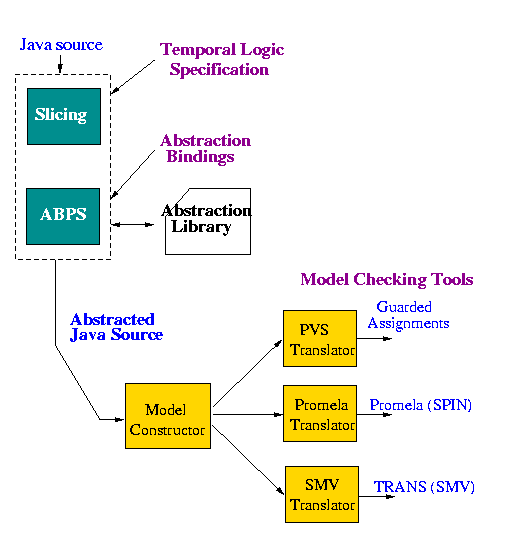
\includegraphics[scale=0.5]{images/bandera_desc.png}
  \caption{\label{fig:desc_bandera_site} Schéma de fonctionnement de Bandera}
   Source: \url{http://bandera.projects.cs.ksu.edu}
\end{figure}


\subsection{Découpage (\textit{slicing}) du programme}
\label{sec:bandera_slicing}

\paragraph{}
Dans le but de ne garder que les instructions intéressantes à la
vérification d'une certaine propriété, Bandera effectue un découpage
des instructions. Pour un programme $P$, des opérations $s_i$ sont
extraites et regroupées dans $C$.

$$C = \{s_1, s_2, \ldots, s_k\}$$

\paragraph{}
Le découpage du programme va réduire $P$ afin de ne laisser que les
instructions nécessaires au bon fonctionnement des opérations
contenues dans $C$, et supprimer les autres.

\paragraph{}
Bandera se sert de cette méthode pour vérifier qu'un programme $P$
adhère à une spécification $\Phi$. Le logiciel supprime les
instructions de $P$ qui n'influent pas la satisfaction de $\Phi$. Si
$\Phi$ est juste pour la version réduite de $P$, alors $\Phi$ est
juste pour la version complète de $P$.

\paragraph{}
Découper un programme permet aussi de simplifier le travail du
vérificateur de modèle en réduisant le nombre d'instructions à
vérifier. Bandera peut ainsi générer un modèle différent en fonction
de la propriété à tester.

\subsection{Abstraction des variables}
\label{sec:bandera_abstraction}

\paragraph{}
Bandera est capable de considérer des variables et méthodes comme
\textit{abstraites}, ce qui signifie que leur valeur concrète n'est
pas spécifiée. Cette abstraction permet de réduire la taille du modèle
et de simplifier le travail du vérifieur.

\paragraph{}
Cette abstraction est effectuée par le \gls{babs}, un composant
spécialisé de Bandera. Lorsqu'une variable est définie abstraite, elle
n'est plus représentée par sa valeur mais par certaines
propriétées. Ces propriétés dépendent de la spécification, par exemple
si une variable de type \verb|ArrayList| est abstraite et qu'on ne
fait que vérifier si une valeur est contenue dedans, elle peut être
remplacée par l'abstraction
$\{ ElementPresentDansListe, ElementAbsentDansListe \}$. Dans ce cas
précis, le \gls{babs} remplacera toutes les actions effectuées sur
l'\verb|ArrayList| par des versions abstraites manipulant des symboles
représentant des deux valeurs possibles, $ElementPresentDansListe$ et
$ElementAbsentDansListe$.

\paragraph{}
Si une opération impossible à représenter par ces deux valeurs est
demandée, par exemple \verb|ArrayList.size()|, alors l'abstraction
renvoie une valeur spéciale notée $\top$. Cette valeur est ensuite
propagée dans le reste du programme, et Bandera s'occupe d'informer le
constructeur de modèle qu'il sera nécessaire d'implémenter un test
non-déterministe quand cette variable sera utilisée.

\subsection{Transformation du code source}
\label{sec:bandera_source}

\paragraph{}
Afin de transformer du code Java en un langage utilisable par des
vérificateurs, Bandera passe par un certain nombre de langages
intermédiaires. Il commence par traduire le programme en Jimple, un
langage utilisé par le framework Soot et établit des correspondances
entre le code Java et le code Soot. Ceci permet au logiciel de
retrouver le n\oe{}ud Java correspondant à n'importe quel n\oe{}ud
dans Jimple.

\paragraph{}
L'arrière-plan (\textit{backend}) de Bandera s'occupe de traduire le
code Jimple en \gls{bir}, un langage bas niveau qui abstrait les
concepts communs à de nombreux logiciels de vérification de modèle. Le
but ce ce langage intermédiaire est de pouvoir ensuite exporter le
\gls{bir} dans différents langages spécialisés pouvant être utilisés
par les vérificateurs de modèles. La traduction est faite par
\gls{birc}. Cette étape intermédiaire est très importante dans la
«~philosophie~» Bandera~: en effet, pour pouvoir exporter le résultat
de l'analyse vers un nouveau vérificateur de modèle, il est seulement
nécessaire d'écrire un greffon pour Bandera convertissant le langage
\gls{bir} en un fichier utilisable par ce nouveau vérificateur.

\paragraph{}
Ce fonctionnement est schématisé dans la figure~\ref{fig:bir_jimple}.

\begin{figure}[H]
  \centering
  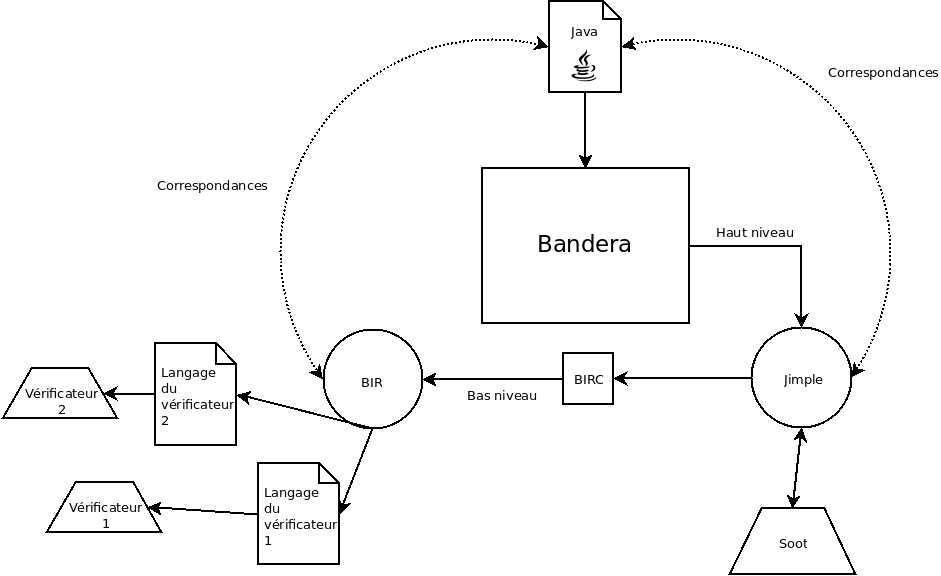
\includegraphics[scale=0.5]{images/bandera_bir_jimple.png}
  \caption{\label{fig:bir_jimple} Transformation du code source en
    langages intermédiaires}
\end{figure}

\section{Interêt et limites}

\paragraph{}
Bandera est un outil très puissant et complexe qui gère même l'analyse
de threads Java. Les développeurs de Bandera ont choisi de ne pas
utiliser JDart (présenté dans la section suivante) pour effectuer
l'analyse afin de pouvoir modifier plus simplement le moteur d'analyse
lorsque de nouvelles avancées seront disponibles. JDart est pourtant
un outil très puissant et toujours maintenu permettant d'analyser des
applications Java.

\paragraph{}
Un des grands points forts de Bandera est de pouvoir exporter le
résultat de son analyse vers de nombreux vérificateurs de
modèle. C'est d'ailleurs son utilisation première, cette application
ayant été développée pour être compatible avec le plus de
vérificateurs possibles.

\paragraph{}
Notre but n'est pas d'écrire un vérificateur de modèle. De plus, afin
de nous simplifier la tâche, nous avons décidé d'utiliser JDart, qui
sera présenté dans la prochaine section. L'API JavaCard ne gérant pas
les threads dans sa version classique (ceux-ci existent dans la
version Connected
Edition\footnote{\url{https://fr.wikipedia.org/wiki/Java_Card#Version_Java_Card_3_.C2.AB.C2.A0Connect.C3.A9e.C2.A0.C2.BB}}),
toute la complexité de Bandera autour de l'analyse des fils
d'exécution ne nous concerne pas non plus.

\paragraph{}
Il apparaît que Bandera est un projet très intéressant pour la
vérification formelle de code. Cependant, la plupart des
fonctionnalités qui nous intéressent --- l'analyse du code, des
changements des variables, etc. --- sont aussi réalisables en
utilisant l'outil JDart, qui sera présenté dans la prochaine
section. Celui-ci est encore maintenu et est plus orienté vers les
développeurs, il sera donc plus simple à intégrer à notre projet.

\paragraph{}
Une autre partie intéressante de Bandera est son utilisation du
framework Soot. Ce dernier est un outil permettant l'analyse et la
modification de code source Java ainsi que de bytecode. Celui-ci
pourrait nous être utile conjointement avec JDart pour extraire les
variables participant aux changements d'état d'un applet JavaCard.


        \chapter{JDart et exécution concolique}
	\paragraph{}
		L'idée générale est de rendre la tâche de tester des Applets Java Card moins penible et plus la plus efficace possible.
		Pour cela nous optons pour l'utilisation de l'exécution concolique comme une technique d'analyse, ce qui permet de rendre 
		le système à tester moins obscur et plus prédictible. Surtout quand on est face à des systèmes complexes
		nécessitant des méthodes plus avancées qu'un simple test unitaire.
    
	\paragraph{}
		\textbf{JDart \footnote{JDart : https://github.com/psycopaths/jdart}} est un outil qui permet d'utiliser l'exécution concolique
		comme une technique de tests pour les applications Java.
		\newline
		Il se présente sous forme d'une extension de \gls{JPF} un outil créé par la NASA afin de tester ses applications, y compris les programmes executés sur ses robots astromobiles.
	\section{Exploration des chemins et l'exécution concolique}
		\subsection{Java Path Finder: Exploration des chemins}
			\nocite{JPF}
			
			\paragraph{}
				\gls{JPF} est un outil de vérification des modèles d'états pour le bytecode Java,
				en réalité \gls{JPF} est une \gls{VM} qui exécute le programme donné en entrée autant de fois que nécessaire
				afin d'explorer chaque chemin qu'il contient.
				
				Tout au long de ce processus, \gls{JPF} collecte les anomalies rencontrées telles que l'interblocage des threads et les exceptions non traitées, puis il génére un rapport contenant les traces qui ménent à ces anomalies.
	
			\begin{figure}[H]
				\centering
					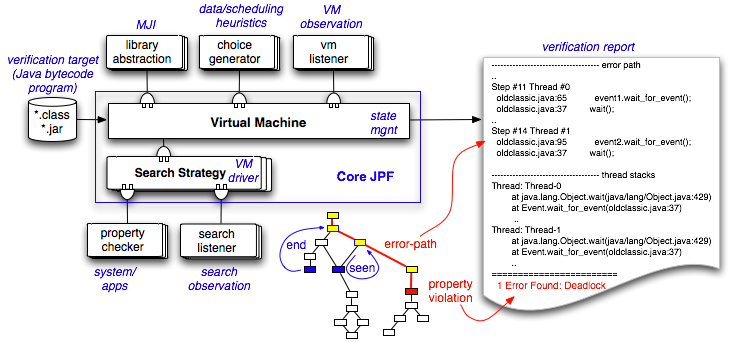
\includegraphics[scale=0.5]{images/jpf-model.png}
				\caption{Modèle d'opération de \gls{JPF}}
			\end{figure}
	
			\paragraph{}
				\gls{JPF} ne se limite pas simplement à détecter les erreurs d'un programme, en effet, il effectue la vérification des modéles.
				C'est un outil qui permet de simuler le non-determinisme. Certains aspects ne peuvent pas être contrôlés par de simples tests et exigent l'assistance d'une \gls{VM}.
				Cependant, en essayant d'explorer et exécuter tous les chemins au sein d'un programme, le nombre d'executions nécessaires peut croître d'une maniére exponentielle (On parle du problème d'explosion d'état). 
				Pour résoudre ce problème, \gls{JPF} réalise une correspondance d'état, c'est un mecanisme qui permet de comparer
				l'état actuel en un n\oe{}ud à des états déjà connus, dans le cas où l'état
				a été verifié \gls{JPF} est capable d'effectuer un retour arrière à la position précédente la plus proche où un chemin inexploré existe et restaure l'état du programme à tester à cette position.
	
			\begin{figure}[H]
				\centering
					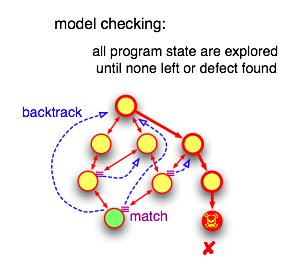
\includegraphics[scale=0.5]{images/jpf-model-checking.png}
				\caption{Vérification du modéles}
			\end{figure}
      
			\paragraph{}
				La vérification des modèles (\textit{Model Checking}) ne dépend pas des conjectures. En théorie si une anomalie est présente dans le programme à tester
				alors la vérification des modéles la trouvera, puisque c'est une méthode qui explore de maniére exhaustive tous les comportements possibles du système ;
				d'où vient l'efficacité du \textit{Model Checking}.
		\subsection{JDart: Exécution concolique}
			\nocite{JDart}
			\nocite{JDart2}

			\paragraph{}
				\gls{JPF} n'est pas une boite noire. L'une des meilleures fonctionalités de \gls{JPF} est la possibilité de le personnaliser entièrement et d'ainsi pouvoir ajouter des extensions facilement.
				Cet aspect a permis la création d'un grand nombre d'extensions utiles comme des moteurs
				qui permettent l'exécution symbolique et concolique.

			\paragraph{}
				Une exécution concolique commence par une entrée concrète, en exécutant le programme à tester, des contraintes symboliques pour les chemins explorés
				sont formés pour cette exécution. Ces contraintes symboliques sont en réalité des formules logiques composées d'un tas de déclarations conditionnelles
				qui ont été collectées tout au long du parcours.

				L'étape suivante consiste à nier une sous formule et donc nous arrivons à créer un nouveau vecteur de valeurs concrétes en utilisant un
				solveur de contraintes.

				Ce vecteur sera utilisé pour une nouvelle exécution du programme ce qui permettra d'éxplorer un nouveau chemin.
				Cette procédure peut être répétée jusqu'à ce que tous les chemins possibles du système à tester soient explorés.
				
			\begin{figure}[H]
				\centering
					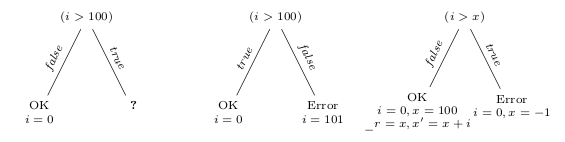
\includegraphics[scale=0.5]{images/concolic.png}
				\caption{Exécution concolique}
			\end{figure}
				
			\paragraph{}
				L'exécution concolique résout un grand problème qui se déclanche généralement au cours de l'exécution concolique, %%Là, je pense qu'il y a une exécution concolique de trop !!!
				puisque l'espace de recherche est réduit significativement de façon à ce que le problème d'explosion d'espace de recherche
				ne peut plus se réaliser car les formules logiques générées par l'execution symbolique indiquera quelle valeur concrète
				doit être fournie pour satisfaire la condition concernée.
				Il n'est plus obligatoire de fournir un grand nombre d'entrées qui, au final, peuvent toutes générer un même chemin.
				\newline
				La technique d'exécution concolique a aussi son effet sur l'exécution symbolique traditionnelle.
				En effet, quand une condition ne peut pas être résolue symboliquement à cause de la complexité de la contrainte (Equation mathématique complexe,
				opération sur les nombres flottant...) elle sera remplacée par une valeur concréte, ce qui permet de continuer l'exploration des chemins.

			\paragraph{}
				JDart est l'une des extensions de \gls{JPF}, il s'agit d'un moteur d'exécution concolique qui traite un programme Java
				en utilisant à la fois des valeurs symboliques et concrétes et garde les traces des exécution symboliques.
				Les formules logiques créées sont ensuite passées à un solveur \textit{\gls{SMT}} afin d'obtenir une évaluation satisfaisante de la contrainte.
				JDart utilise par défaut \textit{\gls{microsoft-z3}} mais  il propose aussi un niveau d'abstraction qui permet d'intégrer d'autres solveurs
				tels que : \textit{Coral} ou \textit{dreal} si nécessaire.
				
			\begin{figure}[H]
				\centering
					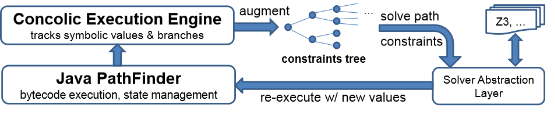
\includegraphics[scale=0.5]{images/archJDart.png}
				\caption{Architecture de JDart}
			\end{figure}
				
			\paragraph{}
				Plus concrètement, la figure~\ref{fig:jdart_sample} montre le résultat d'une portion de code Java executé avec JDart.
				La portion de code admet deux paramétres primitifs et deux simples tests sur ces paramétres, ainsi que la sortie correspondante
				de JDart.
				
			\begin{figure}[H]
				\centering
					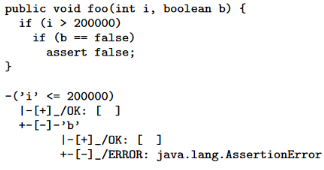
\includegraphics[scale=0.5]{images/jdart_exemple.png}
				\caption{\label{fig:jdart_sample} Exemple d'un programme executé avec JDart}
			\end{figure}
			
			\paragraph{}
				L'arbre des contraintes contient un n\oe{}ud pour chaque condition dans ce fragment de code et deux feuilles.
				Le chemin qui abouti à une erreur est marqué par la classe qui le déclanche.
				Nous n'avons pas affiché les valeurs concrétes qui permettent de parcourir ces chemins, néanmoins, JDart peut être configuré
				de façon à ce qu'il affiche ces valeurs ou génère des tests unitaires basés sur ces valeurs.
      
	\section{La VM JAVA, la VM du JPF et la VM JavaCard}
		\paragraph{}
			Nous avons défini \gls{JPF} comme étant une machine virtuelle qui exécute un code Java et analyse son \textit{\gls{bytecode}},
			
	\section{Tester des applets JavaCard}
	\paragraph{}
		Java Path Finder est connu comme le couteau suisse de la vérification Java,
		il est en effet un des outils de tests les plus évolués pour les applications Java,
		notamment grâce à son extensibilité et à son habilité à supporter et intérger de nouvelle extensions.
		Cependant, la majorité des extensions ne sont pas destinées à être executées sur des systèmes JavaCard.

        \chapter{Génération d'un automate}

\paragraph{}
Dans cette partie nous allons présenter l'outil qui nous permettra de créer 
l'automate d'une applet afin de pouvoir le comparer à l'automate fourni dans les 
spécifications de l'application. Dans nos recherche nous avons trouvé l'outil 
Soot \cite{Soot}.

	\section{Présentation de Soot}

	\paragraph{}
	À l'origine Soot est un framework qui à pour but d'optimiser du code. 
Soot a été produit par le groupe de recherche Sable de l'université de McGill. 
Concrètement ce framework permet de :

	\begin{itemize}
		\item analyser points par points
		\item créer des graphes de séquence
		\item créer des graphes de flux de controle
		\item instrumenter du code
	\end{itemize}

	\paragraph{}
	Soot propose plusieurs représentations intermédiaires du code. Chaque 
représentation intermédiaire correspond à un niveau d'abstraction.

	\paragraph{Baf} est une représentation simplifiée du bytecode Java. Il 
permet de manipuler du bytecode plus simplement.
	\paragraph{Jimple} est la représentation principale de Soot. C'est une 
représentation à trois addresses, c'est-à-dire qu'une instruction peut contenir 
trois variables. Par exemple l'instruction suivante : 
	$$ a = (b + 1) * c - d$$
	Devient : 
	$$ \$i_0 = b + 1$$
	$$ \$i_1 = \$i_0 * c$$
	$$ a = \$i_1 - d$$
	où \$i0 et \$i1 sont des variables intermédiaires.


	Le jeu d'instructions est aussi réduit (15 instructions contre plus de 
200 en bytecode).
	\paragraph{Shimple} est une représentation de type \gls{SSA}, c'est une 
représentation qui interdit la réaffectation d'une variable, des versions de 
variables sont utilisées pour remplir ce critère. Par exemple le code suivant :
	$$ y = 1 $$
	$$ y = 2 $$
	$$ x = y $$
	Devient :
	$$ y_1 = 1 $$
	$$ y_2 = 2 $$
	$$ x_1 = y_2 $$ 
	Cela permet de voir que la première instruction est inutile. Shimple 
permet donc d'éliminer du code mort, de contrôler la propagation de constante...

	\paragraph{Grimp} est une représentation basé sur Jimple, elle 
n'utilise pas de variable intermédiaire ce qui la rapproche plus du langage 
Java. Elle est utiliée pour de la décomplilation ou pour de l'inspection de 
code.

\section{}

\paragraph{}

        \chapter{Représentation et Analyse de graphes}
\paragraph{}

Comme nous l'avons vu auparavant, il est nécessaire de pouvoir stocker les automates générés dans la partie précédente. Pour cela, les graphes nous ont été imposés. Dans cette partie, nous vous présenteront donc les moyens que nous avons à disposition pour réaliser le stockage de graphes et nous les compareront afin d'en sélectionner le meilleur.

\section{Différents format de représentation}
  \paragraph{}
  Il existe de nombreux formats de représentation de graphes tels que le JSON, le CSV ou bien encore l'XML.
  
  Dans cette première partie, nous allons nous concentrer sur le choix du format que nous utiliserons pour stocker et réutiliser nos graphes après leur création dans l'application.
  Nous allons pour cela passer par un tableau comparatif des diverses solutions.
  

  \subsection{Liste des formats de représentation de graphes}
  La liste ci-dessous contient tous les formats de représentation de graphes à comparer : 
  \begin{itemize}
   \item CSV : est un type de fichier très répandu, il représente les informations sous forme de tableaux et est facilement lisible via la plupart des programmes. 
   \item XML : est surement le type de fichier le plus répandu, stockant les donées sous forme de balises, il est très utilisé pour toutes les applications web et orientées objets. 
   \item JSON : le petit nouveau, il est le type de fichier favoris de tous les langages orientés objets car il permet un stockage très simple de tous les types de données, des plus simples aux plus complexes. 
   \item svg : basé sur le XML, ce format est conçu pour supporter les images vectorielles.
   \item bmp : est un format d'image propriétaire lancé par Microsoft, il est assez répandu.
   \item jpg : est un autre format d'image, plus répandu que le bmp.
  \end{itemize}

  
  \subsection{Liste des éléments déterminants le choix}
  Avant de pouvoir comparer les différents types de stockage des graphes, il nous faut déterminer une grille de critères nous permettant de classer les différentes solutions en lice.
  
  La solution retenue devra donc respecter les points suivants : 
  \begin{itemize}
   \item utiliser un format libre de données.
   \item assurer la portabilité des information en étant lisible par le plus grand nombre d'applications.
   \item être simple de lecture et de traitement, tirer facilement un graphe sous forme graphique des données stockées.
   \item facilement modifiable : si on souhaite rajouter des éléments au graphe
   \item supporter le langage objet nativement, car l'automate généré sera représenté sous forme d'objet et les graphes le seront également.
  \end{itemize}
  
  \begin{table}[!h]{Tableau comparatif des formats de fichiers}
  \centering
    \begin{tabular}{p{3.5cm} p{0.50cm} p{0.5cm} p{0.50cm} p{0.5cm} p{0.50cm}}

	& \makebox[0cm][l]{\rotatebox{45}{ Format libre }} &
	\makebox[0cm][l]{\rotatebox{45}{ Inter langages }} &
	\makebox[0cm][l]{\rotatebox{45}{ Conversion en image simple}} &
	\makebox[0cm][l]{\rotatebox{45}{ Évolution simple }} &
	\makebox[0cm][l]{\rotatebox{45}{ Support objet natif }}\\
	    
    \end{tabular}
    
    \begin{tabular}{|p{3.5cm} | p{0.50cm} | p{0.5cm} | p{0.50cm} | p{0.5cm} | p{0.50cm} |}
      
      \hline  
      \textbf{CSV}	& x & x & x & x &	\\ \hline
      \textbf{XML} 	& x & x & x & x & x 	\\ \hline
      \textbf{JSON} 	& x & x & x & x & x 	\\ \hline
      \textbf{SVG} 	& x & x & x &	& x 	\\ \hline
      \textbf{BMP} 	& x & x & x &  	&  	\\ \hline
      \textbf{JPG} 	& x & x & x &  	&  	\\ 
      \hline
    \end{tabular}
  \end{table}
  
  \subsection{Bilan}
  Après comparaison, nous voyons que deux formats peuvent correspondre à notre attente : l'XML et le JSON, nous allons donc nous baser sur ces résultats pour rechercher un outil nous permettant de représenter les graphes à l'aide d'un de ces formats.

  \section{Outils de représentation existants}
  
  \paragraph{}
  Après avoir déterminé les formats de fichiers les plus appropriés, il nous faut encore trouver un outil servant à représenter et dessiner les graphes ou, si nous n'en trouvons pas un qui conviendrait, se servir d'un outil pour base afin de le modifier en implémentant les fonctions recherchées.
  
  \subsection{Fonctionnalités demandées et contraintes imposées}
  Pour répondre à tous nos besoins, la solution retenue devra implémenter les fonctionnalités suivantes : 
  \begin{itemize}
  	\item Proposer une sortie simple à comprendre pour l'utilisateur
  	\item Dessiner un graphe à partir d'un fichier source
  \end{itemize}
  
  \paragraph{}
  La solution retenue devra également répondre aux contraintes suivantes : 
  \begin{itemize}
  	\item Posséder une licence libre afin de pouvoir apporter d'éventuelles modifications au code source.
  	\item Être intégrable à notre application finale.
  	\item Être facilement maintenable dans le futur.
  \end{itemize}

  \begin{longtable}{|c|p{2cm}|p{2cm}|p{8cm}|}
    \caption{Quelques solutions possibles de représentation de graphe et leur description}\\
    \hline
    \textbf{Nom} & \textbf{Langage} & \textbf{Licence} & \textbf{Description} \\
    \hline \hline
    
    \endfirsthead
    \hline
    \textbf{Nom} & \textbf{Langage} & \textbf{Licence} & \textbf{Description} \\
    \hline \hline
    
    \endhead
	
    \textbf{Dracula \footnote{Dracula : https://www.graphdracula.net/}} & 
JavaScript & MIT & Dracula est une bibliothèque très simple à utiliser par les 
utilisateurs, des options de drag-and-drop y sont présentes. Côté développeur, 
les fonctions d'ajout de n\oe{}uds et de gestion globales des graphes ont été 
implantées ainsi que certains algorithmes commums (Dijkstra, divers 
parcours...)\\
    \hline
    \textbf{Graph\footnote{Graph :  https://github.com/clue/graph}}& PHP & MIT &  Graph est une bibliothèque créée pour représenter des graphes, l'utilisation de PHP permet de créer un affichage minimaliste et simple en réalisation en raison de l'utilisation des navigateurs webs. Cependant, il est nécessaire de mettre en place un serveur PHP, et ceci est une opération trop lourde pour être utilisée à grande échelle.\\
    \hline
    \textbf{MXGraph\footnote{MXGraph : https://www.jgraph.com/}}& JavaScript &  Apache 2.0 & MXGraph utilise un rendu SVG pour représenter les graphes, ce qui est un gros avantage, car si les graphes obtenus sont très complexes, il est toujours possible de zommer sur une zone sans perdre en lisibilité.\\
    \hline
    \textbf{JGraphx\footnote{JGraphx : https://github.com/jgraph/jgraphx}}&Java& BSD 3 & JGraphx est développé par les mêmes personnes que MXGraph, mais contrairement à ce dernier, JGraphx utilise Java Swing comme sortie. Java Swing étant en fin de vie et très difficile à adapter, cette solution est à écarter. \\
    \hline 
    \textbf{GraphStream\footnote{GraphStream : http://graphstream-project.org/}}& Java & LGPL v3.0 & GraphStream est une bibliothèque Java avec une sortie très poussée prévue pour gérer de gros graphes. Cette solution est donc accessible pour l'utilisateur, du côté développeur, le fait que la bibliothèque soit développée en Java est un gros avantage pour l'intégration à l'application. \\
    \hline
  \end{longtable}
  
  \subsection{Comparaison des bibliothèques disponibles}
  
    \begin{table}[!h]{Tableau comparatif des bibliothèques}
      
      \centering
    
    \begin{tabular}{p{3.5cm} p{0.50cm} p{0.5cm} p{0.50cm} p{0.5cm} p{0.5cm} p{0.5cm} }

	& \makebox[0cm][l]{\rotatebox{45}{ Format libre }} &
	\makebox[0cm][l]{\rotatebox{45}{ Intégration simple }} &
	\makebox[0cm][l]{\rotatebox{45}{ User-friendly}} &
	\makebox[0cm][l]{\rotatebox{45}{ Dessin à partir d'un fichier }} &
	\makebox[0cm][l]{\rotatebox{45}{ Maintenabilité }}&
	\makebox[0cm][l]{\rotatebox{45}{ Classement }}\\
	    
    \end{tabular}
    
    \begin{tabular}{|p{3.5cm} | p{0.50cm} | p{0.5cm} | p{0.50cm} | p{0.5cm} | p{0.5cm}| p{0.5cm}|}
      
      \hline  
      \textbf{Dracula} 		& x & x 			& \textcolor{green}{+}	& N/I	& \textcolor{green}{+}	& 2\\ \hline
      \textbf{Graph} 		& x & \textcolor{red}{-} 	& \textcolor{red}{-} 	& N/I 	& \textcolor{red}{-}	& 4\\ \hline
      \textbf{MXGraph} 		& x & x 			& x 			& N/I 	& \textcolor{green}{+}	& 3\\ \hline
      \textbf{JGraphx} 		& x & \textcolor{red}{-} 	& \textcolor{red}{-} 	& N/I 	& \textcolor{red}{-}	& 4\\ \hline
      \textbf{GraphStream} 	& x & \textcolor{green}{+}	& \textcolor{green}{+} 	& N/I 	& \textcolor{green}{+}	& \textbf{1}\\ 
      \hline
    \end{tabular}
    
    \begin{tabular}{c c c}
    &&\\
    x : normal & + = avantage & - = inconvénient\\
    N/I : non-implémenté & \textcolor{green}{vert} = avantage & \textcolor{red}{rouge} = inconvénient\\
    \end{tabular}

  \end{table}
  
  \subsection{Bilan}
  La solution retenue est la solution GraphStream, qui semble être celle convenant la plus aux attentes. Dans tous les cas, nous aurons à implémenter l'importation de graphes à partir de fichiers.
  
  Si au cours du développement nous nous rendons compte de l'impossibilité de nous interfacer avec GraphStream, nous aurons la possibilité de migrer vers Dracula qui est le second choix le plus intéressant.
  

  \section{Outils d'analyse existants}

  \paragraph{}
  Après avoir réussi à représenter les graphes extraits des sorties de JDart, il nou faut encore un outil capable d'analyser les graphes afin de pouvoir simplifier leur conversion en automates.

  \subsection{Description des solutions en lice}
  \paragraph{}
  Pour cette tâche, trois solutions ont été retenues, nous allons, dans cette partie réaliser un bref comparatif de chacune d'entre elles afin de déterminer laquelle permet de répondre au mieux à nos attentes.
  
  \begin{longtable}{|c|p{2cm}|p{2cm}|p{8cm}|}
    \caption{Quelques solutions d'analyse de graphe possibles et leur description}\\
    \hline
    \textbf{Nom} & \textbf{Langage} & \textbf{Licence} & \textbf{Description} \\
    \hline \hline
    
    \endfirsthead
    \hline
    \textbf{Nom} & \textbf{Langage} & \textbf{Licence} & \textbf{Description} \\
    \hline \hline
    
    \endhead
	
    \textbf{Medusa (I) \footnote{Medusa :  http://bioinformatics.oxfordjournals.org/content/21/24/4432.short}} & Java & Inconnue & Medusa est un outil de traitement des graphes destiné à décomposer et reconnaître des protéines ou des gènes. Il est composé d'une interface graphique et d'un c\oe{}ur tous deux codés en Java. Cependant, il a l'air compliqué, à priori, d'adapter cet outil à notre type d'utilisation.\\
    \hline
    \textbf{Graph-Tool \footnote{Graph-Tool : https://graph-tool.skewed.de/}}& Python/C++ & GPLv3 &  Graph-Tool est un outil très complet d'analyse et de génération de graphes, même si la partie génération n'est pas celle qui nous intéresse le plus, la partie analyse reste néanmoins assez étoffée. Elle permet, en autres, de calculer l'isomorphisme d'un graphe, l'arbre couvrant minimal, les composantes connexes. \\
    \hline
    \textbf{Gephi \footnote{Gephi :  https://gephi.org/publications/gephi-bastian-feb09.pdf}}& Java &  GPLv3 & Gephi est un logiciel Open Source implémentant une interface graphique ainsi qu'un c\oe{}ur en Java. Il permet de réaliser de nombreuses représentations de graphe ainsi que d'appliquer de nombreux calculs sur ces derniers. L'interface grahique n'étant pas notre priorité dans cette partie, il reste à noter qu'il nous sera toujours possible de nous en inspirer pour l'adapter. \\
    \hline
    \textbf{Medusa (II) \footnote{Medusa :  https://github.com/JianlongZhong/Medusa}}& Cuda/C++ &  BSD 3 & Homonyme du premier logiciel présenté, il est tout de même très différent de ce dernier : de par le langage utilisé pour le développer, CUDA à la place de Java, d'une part. Par son objectif beaucoup plus adaptatif et polyvalent, d'autre part. \\
    \hline
  \end{longtable}
  
  \paragraph{Bilan post-présentation}
  Après la présentation des différentes solutions possibles, il semble logique d'éliminer  Medusa (I) pour des raisons d'adaptabilité trop complexe à mettre en place.
  
  \subsection{Comparaison des solutions possibles}
  
  \paragraph{}
  Il nous reste donc à départager les trois solutions restantes : 
  \begin{itemize}
  	\item Graph-Tool
  	\item Gephi
  	\item Medusa
  \end{itemize}

    
    \begin{table}[H]
      
      \centering
    
    \begin{tabular}{p{3.5cm}  p{6cm}  p{6cm} }

	& \textbf{Avantages} 		& \textbf{Inconvénients}\\ 
    	
    \end{tabular}

    
    \begin{tabular}{|p{3.5cm} | p{6cm} | p{6cm} |}
      
      \hline
      \textbf{Graph-Tool} 	& Haute performance grâce à son c\oe{}ur en C++, nombreuses fonctionnalités déjà implémentées	
				& Difficulté d'intégration en raison du langage. \\ \hline
      \textbf{Gephi} 		& Certainement plus simple à intégrer à notre application en raison de son codage en Java. Nombreuses fonctionnalités déjà implémentées.
				& Contient des outils non indispensables : la GUI par exemple, ce qui rajoutera certainement une difficulté d'extraction des fonctions pouvant nous intéresser. 	\\ \hline
      \textbf{Medusa} 		& Très hautes performances sur les graphes de grande taille grâce à son parallélisme. Nombreuses fonctionnalités déjà implémentées.
				& Uniquement compatible avec du matériel Nvidia, difficulté d'intégration en raison du langage.	\\ \hline
    \end{tabular}

    \caption{Avantage et inconvénient des différents outils }
  \end{table}
  
  
  \subsection{Bilan}
  
  \paragraph{}
  Après avoir présenté les différentes solutions et établi une comparaison sommaire, il ressort que les trois solutions sont relativement équivalentent sur les fonctionnalités proposées. Seuls les langages et les manières d'arriver au résultat diffèrent.
  
  \paragraph{}
  Dans notre problématique, nous n'aurons certainement pas à gérer de trop gros graphes, en effet, bien que complexes, les applets JavaCard sont limités en taille (contrainte naturelle d'une carte à puce). Ayant également une contrainte de temps, il semble logique de préférer la solution codée en Java, nous aurons ainsi plus de simplicité à l'intégrer à notre application finale.
  
  \paragraph{}La solution retenue dans cette partie est donc \textbf{Gephi}.
  
  \section{Bilan global de la partie Graphes}
  
  \paragraph{}
  Dans ce chapitre, nous avons vu plusieurs formats de fichiers et outils permettant de répondre au problème de gestion de graphes.
  
  Nous avons donc choisi d'utiliser le format JSON pour stocker nos graphes, de nombreux outils en Java permettent de gérer simplement ce format, il y aura donc moins de travail à fournir de ce point de vue là.
  
  Concernant l'outil de représentation des graphes, GraphStream sera celui utilisé en priorité, il permettra un affichage clair et une interaction avec l'utilisateur.
  
  Pour terminer, Gephi permettra d'appliquer des traitements sur les graphes pour en tirer le maximum d'informations.
  
  


        \chapter{Tâches futures et planification}

\section{Outils qui seront utilisés pour la réalisation du projet}
\subsection{Gestionnaire de version}
\paragraph{}
Pour la réalisation de ce projet, il nous a été demandé d'utiliser un gestionnaire de version.

La Direction des Systèmes d'Information ayant mis en place un serveur Git à disposition des étudiants, les responsables du module nous ont demandé de l'utiliser.

\paragraph{}
Un gestionnaire de version nous permettra d'optimiser notre temps de travail en réduisant les regressions de code, ou en permettant de travailler simultanément sur plusieurs facettes de notre application en utilisant le système de branches.

\subsection{Gestionnaire de dépendances}
\paragraph{}
Pour gérer les dépendances de notre projet, nous avons choisi d'utiliser Maven, il s'agit d'un logiciel simplifiant la gestion des dépendances et des versions de chacune d'entre elles.

\paragraph{}
Lors du clonage de notre projet, il suffira donc, théoriquement tout du moins, de laisser Maven configurer les dépendances pour que tut fonctionne simplement.

\subsection{}

\section{Plannification de l'avancement du projet au semestre 2}

\shorthandoff{:!}
\begin{figure}[H]
  \centering
  \begin{ganttchart}[
    vgrid,hgrid,
    title height=1
    ]{2}{31}
    \gantttitle{Janvier}{6}  \gantttitle{Février}{6} \gantttitle{Mars}{6} \gantttitle{Avril}{6} \gantttitle{Mai}{6} \\
    \gantttitlelist{6,11,16,21,26,31}{1} \gantttitlelist{3,8,13,18,23,28}{1} \gantttitlelist{6,11,16,21,26,31}{1} \gantttitlelist{5,10,15,20,25,30}{1} \gantttitlelist{6,11,16,21,26,31}{1} \\
    \ganttgroup{Group 1}{2}{7} \\
    \ganttbar{Task 1}{2}{2} \\
    \ganttlinkedbar{Task 2}{3}{7} \ganttnewline
    \ganttmilestone{Milestone}{7} \ganttnewline
    \ganttbar{Final Task}{8}{12}
    \ganttlink{elem2}{elem3}
    \ganttlink{elem3}{elem4}
  \end{ganttchart}
\caption{Planning prévisionnel du second semestre}
\end{figure}

\section{Quelles tâches à effectuer au semestre prochain ?}
\section{Tableau de planification des tâches}
        
	\chapter*{Conclusion}

\paragraph{}
Tout au long de ce semestre, nous avons réalisé une étude de documents et de solutions possibles pour mener à bien la réalisation de notre projet lors du second semestre.

\paragraph{}
Après réalisation de ce travail, nous avons en notre possession les outils nécessaires à la bonne tenue du projet. Après avoir déterminé les différentes tâches de notre projet et avoir déouper ces dernières en sous tâches précises, nous avons également une bonne idée quant aux travaux que nous aurons à réaliser après le dépôt de ce rapport. 

\paragraph{}
L'étape de réflexion qu'a été la rédaction de ce rapport nous a permis de prendre du recul vis-à-vis de l'énoncé qui nous avait été donné au début de l'année. Ce recul nous permet de débuter la phase de réalisation de manière sereine, nous savons où nous allons et quelles étapes sont à parcourir. De plus, en cas d'imprévu, nous avons vu suffisamment de solutions et de techniques différentes pour pouvoir nous adapter si besoin.

\paragraph{}



    %Glossaire des Acronymes
    %\printglossary[type=\acronymtype]
    %Glossaire
    \glossarystyle{altlist}
    \printglossary[type=\acronymtype]
    \printglossary
    
    \clearpage 
    \bibliographystyle{plain}
    \bibliography{bibliographie}
    \addcontentsline{toc}{section}{Références}


\end{document}